Le but de ce TP est d'étudier différentes structures au moyen d'ondes de Lamb.
L'objectif premier est de comprendre la génération des ondes de Lamb (au moyen d'un
faiseau ultrasonore d'une part et de la technologie EMAT\footnote{ElectroMagnetic Acoustic
Transducer} d'autre part), l'objectif second est de déterminer comment ces ondes peuvent être utilisées pour détecter des défauts dans des structures complexes.

Ce TP se décompose ainsi en trois parties :
\begin{enumerate}
    \item Approche théorique du phénomène
    \item Mesure des ondes de Lamb sur une plaque
    \item Positionnement de défauts sur une conduite par ondes de Lamb
\end{enumerate}

\section{Ondes de Lamb -- Élements de Théorie}

Les ondes de Lamb sont des ondes se propageant dans toute l'épaisseur d'une plaque, leurs multiples réflections sur les surfaces de la plaque en font un outil précieux pour la détection de défaut.

Ces ondes présentent deux comportements modaux distincts\footnote{Symétrique et Antisymétrique} et répondent à l'équation~\eqref{emat:eq_lamb}.
En cherchant les racines de chacun des deux termes de l'équation, il est possible d'obtenir les courbes de dispersion des différents modes et donc de savoir lesquels sont excités pour une fréquence donnée.

\begin{floatEq}
    \begin{equation}
        \begin{array}{c}
        \overbrace{
        \left[4k_x^2k_{z_L}k_{z_T}\cos\left( k_{z_L}\frac{h}{2}\right)\sin\left(k_{z_T}\frac{h}{2}\right) +\left( 2k_x^2-k_T^2\right) ^2\cos\left( k_{z_T}\frac{h}{2}\right)\sin\left( k_{z_L}\frac{h}{2}\right) \right]}^{\mathrm{modes~symétriques}}\\
        \cdot\underbrace{\left[4k_x^2k_{z_L}k_{Z_T}\cos\left( k_{z_T}\frac{h}{2}\right) \sin\left( k_{z_L}\frac{h}{2}\right) +\left( 2k_x^2-k_T^2\right) ^2\cos\left( k_{z_L}\frac{h}{2}\right) \sin\left( k_{z_T}\frac{h}{2}\right) \right]}_{\mathrm{modes~antisymétriques}}=0
        \end{array}
        \label{emat:eq_lamb}
    \end{equation}
\end{floatEq}

Les courbes de dispersion pour une plaque d'aluminium (dont les paramètres sont disponibles en table~\ref{emat:params_alu}) sont présentées dans le plan $(fh,v_\phi)$ en Figure~\ref{emat:disper_alu}.

\begin{figure}
	\centering
	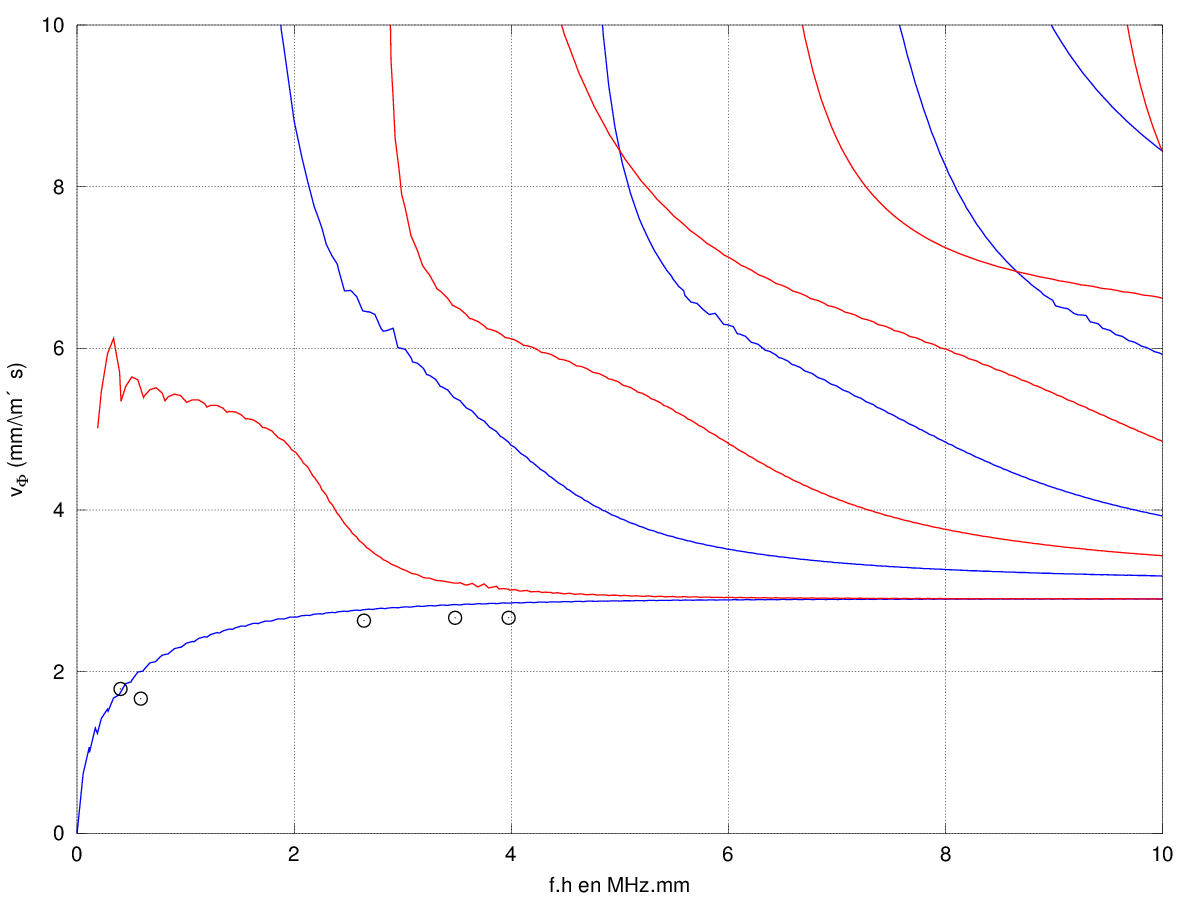
\includegraphics[width=0.8\linewidth]{me_figs/dispercurves_aluminium.png}
	\caption{Courbes de dispersion théoriques pour une plaque d'aluminium de 5.6mm
	d'épaisseur. Les modes symétriques sont en bleu, les antisymétriques en rouge. Les
	marques noires correspondent aux mesures présentées en~\ref{emat:sec:oscillo}.}
	\label{emat:disper_alu}
\end{figure}

La théorie de Lamb~\autocite{lamb_waves_1917} a été développée pour des plaques infinies
dans le plan, plongées dans le vide. La propagation d'ondes de Lamb dans une plaque finie induit des réflexions sur les bords de la plaque. Ces ondes réfléchies forment une traînée diffuse lors de la mesure. Il est par conséquent difficile (voir~\ref{emat:sec:oscillo}~) de mesurer et suivre les différentes ondes se propageant. Afin de simplifier l'étude expérimentale, seule une fenêtre assez courte est considérée pertinente (avant que les modes ne s'entre-masquent).


\begin{table*}[t]
    \centering
    \begin{tabular}{l|cc}
        Paramètre & Valeur & Unité\\\hline
        Vitesse de l'onde longitudinale dans l'acier $v_L$ & $6450$ & $m.s^{-1}$\\
        Vitesse de l'onde transversale dans l'acier $v_T$ & $3100$ & $m.s^{-1}$\\
        Épaisseur de la plaque $e$ & $5.6\cdot 10^{-3} \pm 0.1\cdot 10^{-3}$ & $m$\\
    \end{tabular}
    \caption{Paramètres de la plaque en aluminium.}
    \label{emat:params_alu}
\end{table*}

\section{Mesure des ondes de Lamb sur une plaque}
\subsection{Montage}

Les transducteurs disponibles étaient centrés à 0.5MHz et 1MHz.

Dans un premier temps, les ondes étaient générées à l'aide d'un transducteur placé au contact\footnote{Avec du couplant} de la surface, en incidence normale.
La condition de fenêtre d'analyse courte évoquée plus haut impose que la distance entre les transducteurs ne soit pas trop grande.

\begin{figurehere}
\begin{tikzpicture}[>=stealth]
    \def\platehalfwidth{3}
    \newcommand\transducer[2]{
        \draw[thick] (#1+0,0) rectangle ++(.3,.4);
        \draw[thick] (#1+.15,.4) .. controls (#1+.2,.7) and (#1+.3,.7) .. (#1+.3,1);
        \draw (#1+.15,0) node[below] {#2};
    }
    \newcommand\inp[3]{
        \draw (0+#1,0+#2) -- ++(.2,0) -- ++(-.1,.2) -- cycle;
        \draw (.3+#1,.6+#2) node[rotate=90, above] {#3};
    }

    % part
    \draw[very thick] (-\platehalfwidth,0) -- (\platehalfwidth,0);
    \draw[very thick] (-\platehalfwidth,-1) -- (\platehalfwidth,-1);
    \draw[very thick] (-\platehalfwidth,0) .. controls (-\platehalfwidth-.5,-.5) and (-\platehalfwidth+.5,-.5) .. (-\platehalfwidth,-1);
    \begin{scope}[shift={(2*\platehalfwidth,0)}]
        \draw[very thick] (-\platehalfwidth,0) .. controls (-\platehalfwidth-.5,-.5) and (-\platehalfwidth+.5,-.5) .. (-\platehalfwidth,-1);
    \end{scope}

    % transducers
    \transducer{\platehalfwidth{}-1.5}{$TX$}
    \transducer{\platehalfwidth{}-4}{$RX_1$}
    \transducer{\platehalfwidth{}-5.5}{$RX_2$}

    % distances
    \draw[<->] (\platehalfwidth-4,.2) -- ++(-1.2,0)  node[midway, above] {$25mm$};
    \draw[<->] (\platehalfwidth-1.5,.2) -- ++(-2.2,0)  node[midway, above] {$50mm$};

    % GBF
    \draw[very thick] (.5,2.5) -- ++ (0,-.5) -- ++(2,0) -- ++(0,.5) node[midway, right] {GBF};
    \inp{1}{2}{SYNC}
    \inp{1.7}{2}{OUT}

    % Oscillo
    \draw[very thick] (-1.8,2.5) -- ++ (0,-.5) node[midway, left] {Oscilloscope} -- ++(2,0) -- ++(0,.5);
    \inp{-.3}{2}{TRIG}
    \inp{-0.8}{2}{CH1}
    \inp{-1.3}{2}{CH2}

    % cables
    \draw[thick] (1.1,2) -- ++(0,-.3) -- (-.2,1.7) -- ++(0,.3);
    \draw[thick] (1.8,2) -- (1.8,1);
    \draw[thick] (-.7,1) -- (-.7,2);
    \draw[thick] (-2.2,1) -- ++(0,.5) -- (-1.2,1.5) -- ++(0,.5);

    % dimensions
    \draw[<->] (2.5,0) -- ++(0,-1) node[midway, right] {$e$};
\end{tikzpicture}
\caption{\label{emat:dispositif_plaque}Dispositif de mesure de la vitesse de propagation des différents modes de Lamb dans une plaque avec un oscilloscope et un générateur de signaux.}
\end{figurehere}

\subsection{Mesures à l'oscilloscope}\label{emat:sec:oscillo}

Le signal d'excitation utilisé est un \textit{burst}, de 3 cycles de sinusoïde sur une fenêtre de 10ms.

L'utilisation d'une période de répétition du \textit{burst} assez grande permet de
s'affranchir des problèmes liés à la superposition de signaux d'excitation. Dans toutes
les mesures, l'ensemble du train d'ondes ne couvrait pas plus de 5 à 10\% de la période de
répétition totale.

En superposant les signaux venant de $RX_1$ et $RX_2$ sur l'oscilloscope il est alors
possible de mesurer le temps de parcours du signal entre les deux récepteurs et de
remonter alors à la vitesse de propagation (vitesse de phase) pour chacun des mode
distingables.

Le système expérimental en place, différentes mesures de temps de vol entre $RX_1$ et
$RX_2$ à différentes fréquences sont réalisées.


La vitesse de chacun des modes de Lamb dépend grandement de la fréquence. De même, dans
l'espace $(fh,v_\phi)$, les courbes de dispersion s'entre-croisent : sans
connaissance \textit{a priori} de ces courbes, il n'est pas possible d'identifier un mode
particulier (l'orde d'arrivée change).

De plus, avec l'augmentation de la fréquence, les vitesses des différents modes convergent vers la même asymptote. Si au début de l'analyse il est possible d'observer des ondes bien séparées, cela devient vite impossible et un seul paquet est observable sans que des modes particuliers soient vraiment distingables.

Les résultats les plus probants des mesures réalisées sont présentés sous forme de cercles
noirs sur la figure~\ref{emat:disper_alu}.

L'adéquation entre la courbe de dispersion et le mode S0 est plutôt bonne mais les autres
mesures étaient toutes largement en dessous de l'asymptote commune.

La mesure précise d'ondes de Lamb avec un oscilloscope est un exercice complexe notamment
à cause des variations importantes de vitesse en fonction de la fréquence et de
l'épaisseur.

Dans la suite un système EMAT sera utilisé. Ces éléments ont notamment l'énorme avantage
de pouvoir générer un mode de Lamb particulier plutôt que tous les modes en même temps
(comme c'était le cas précédement).

\section{Mesures EMAT}

La méthode de mesure utilisée dans la suite est basée sur le système EMAT\footnote{\textit{Electromagnetic Acoustic Transducer}}. Le principe est de générer des ondes acoustiques dans un matériau ferro-magnétique au moyen d'un champ electromagnétique.

Le système EMAT se compose donc d'un chariot porteur d'une bobine au pas calibré pour exciter certains modes de la pièce et d'un odomètre. Le tout est relié a un boîtier de contrôle et, éventuellement à un ordinateur pour automatiser les acquisitions et faciliter le traitement.

Dans le cas présent, le logiciel de contrôle (et d'export) normalement disponible sur l'ordinateur associé n'était pas fonctionnel. Le système chariot/boîtier a pour seul format de sortie des fichiers .dat qui s'avèrent être des binaires non documentés.

Malgré beaucoup de bonne volonté, tous les efforts pour accèder aux données présentes dans le binaire se sont montrés quasi-infructueux. Au mieux, il a été possible de récupérer des méta-données sur l'acquisition et une forme de signal temporel sans indice d'échelle temporelle ou en amplitude.

Sans pouvoir faire mieux dans le temps imparti, l'option choisie est de ne pas considérer les mesures réalisées et de proposer simplement un protocole possible pour détecter et positionner des défauts au moyen d'un système EMAT dans une pièce cylindrique.

\subsection{Interaction entre défauts et ondes}

Les ondes de Lamb se propagent dans toute l'épaisseur du matériau et leur vitesse de phase dépend de cette épaisseur (voir équation~\eqref{emat:eq_lamb} et noter la dépendance en $h$). La présence d'un défaut modifie l'épaisseur (corrosion, fissure débouchante) ou induit une discontinuité dans l'espace de propagation (fissure non-débouchante).

Dans le second cas, la discontinuité provoque une réflexion de l'onde visible sur la trace
temporelle (voir figure~\ref{emat:ondes_conduite}). Dans le premier cas, la modification de l'épaisseur change la constante de propagation (liée à la vitesse) et par conséquent provoque un changement d'impédance plus ou moins brusque et donc une réflexion plus ou moins marquée.

Dans ces deux cas, la conclusion est qu'une réflexion dans la trace est liée à un défaut. Exception doit être faite toutefois des discontinuités liées à des composantes géométriques particulière (épaulements, perçages, etc...) que l'opérateur consciencieux prendra bien évidemment en considération dans son analyse.

\begin{figure}
	\centering
	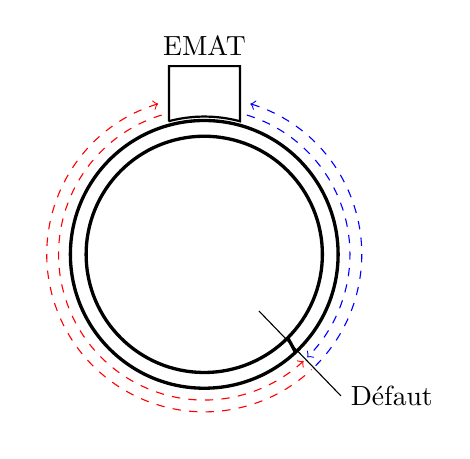
\begin{tikzpicture}
		% tube
		\draw[very thick] (0,0) circle (1.5);
		\draw[very thick] (0,0) circle (1.7);

		% EMAT
		\draw[thick] (105:1.75) arc (105:75:1.75) -- ++(0,.7) -- ++(-.9,0) node[midway, above] {EMAT} -- ++(0,-.7);

		% crack
		\draw[very thick] (-45:1.5) -- (-47:1.7);
		\draw[thin] (-46:1) -- (-46:2.5) node[right] {Défaut};

		% ondes horaires
		\draw[dashed, blue,->] (73:1.85) arc (73:-45:1.85);
		\draw[dashed, blue,<-] (73:2) arc (73:-45:2);

		% onde anti-horaires
		\draw[dashed, red,->] (107:1.85) arc (107:313:1.85);
		\draw[dashed, red,<-] (107:2) arc (107:313:2);

	\end{tikzpicture}
	\caption{Des ondes de Lamb se propagent au sein de la conduite de par et d'autre de
	l'EMAT. Le défaut produit une réflexion précoce et sur la base des temps de vol
	aller-retour il peut être positionné.}
	\label{emat:ondes_conduite}
\end{figure}

\paragraph{Position relative chariot/défaut}
Le temps de vol de l'onde réfléchie renseignant sur la distance entre le chariot de mesure et le défaut, il est alors logique que deux mesures (loin des défauts) suffisent à détecter et positionner un défaut.

Cette clause portant sur le fait que le chariot ne soit pas positionné sur ou trop proche d'un défaut est liée à l'existence de zones mortes (comme pour la méthode TOFD\footnote{\textit{Time Of Flight Difraction}}).
Contrairement au cas le plus idéal, l'émission du signal d'excitation n'est pas un évènement infiniment court et l'émission masque, pendant un temps significatif, toute réflexion précoce.

Afin de s'affranchir de ce problème, il est envisageable de réaliser trois et non deux mesures sur la pièce à des angles différents et d'opérer un recoupement des données ensuite. Le choix des angles doit se faire en considérant la géométrie de la pièce, ses défauts éventuellement visibles, etc. Il sera peut être également nécessaire d'envisager des angles réparti inégalement ou même de refaire des mesures plus précise autour de défauts détectés pour affiner l'analyse.

\paragraph{Différents Modes}
Différents modes de Lamb se propagent \textit{a priori} à différentes vitesses (jusqu'à une certaine fréquence)  et n'induisent pas les mêmes contraintes internes. Par conséquent, différents modes ne réagiront \textit{a priori} pas de la même manière avec différents défauts. Il est alors judicieux de réaliser des mesures en excitant différents modes.

\subsection{Mode Opératoire}

Considérant les différents points évoqués au paragraphe précédent le mode opératoire pour un contrôle de conduite par EMAT pourrait être :

\begin{enumerate}
    \item Analyser la géométrie de la pièce et déterminer 3 axes possibles pour l'avance du chariot sur toute la longueur de la section à contrôler.
    \item Opérer une mesure blanche pour contrôler le bon fonctionnement du système sur une pièce (ou une section) considérée saine.
    \item Réaliser une mesure sur chacun des axes d'avance prévus, noter les angles relatifs entre les passes.
    \item Refaire une mesure par axe pour au moins deux autres modes de Lamb.
    \item Afficher des images d'ensemble pour chaque mode de Lamb excité et constater la position des défauts.
    \item Refaire des mesures autour des défauts avec différents modes de Lamb pour améliorer la caractérisation du défaut.
\end{enumerate}

\newpage

\section*{Conclusion}

Les ondes de Lamb présentent un grand nombre d'intérêts ; en effet leur sensibilité aux changements d'épaisseur du milieu de propagation est un avantage considérable pour le CND appliqué à des conduites.

L'utilisation de systèmes EMAT permet d'exciter un mode particulier du système sans action mécanique sur la pièce. Ce point est particulièrement avantageux dans le cas de systèmes critiques où un dommage minime peut avoir des conséquences dramatiques (\textit{pipelines}, conduites chimiques etc.).

La précision que démontrent les EMAT dans la génération de modes particuliers du système pourrait être couplée à des techniques de traitement de signal avancé pour la détection de forme. En ajoutant à l'équation un système expert avec apprentissage supervisé, il serait peut être possible d'aboutir à un outil capable de mesurer et caractériser automatiquement des défauts qui ne demanderait qu'un minimum d'action humaine.
Cette optique prend tout son sens dans le cas de système de SHM\footnote{Structure Health Monitoring}.
